\documentclass{article}
\usepackage{fullpage}
\usepackage{sectsty}
\usepackage{color}
\usepackage{enumerate}
\usepackage{graphicx, subfigure}
\usepackage{amsfonts, amsmath, amsthm, bm, amssymb}

\usepackage{macro}
\usepackage[utf8]{inputenc}
\usepackage[normalem]{ulem}
\usepackage{lipsum} % for sample text
\usepackage{changepage} % for the adjustwidth environment
%\sectionfont{\large}
\usepackage{color}

\newcommand{\defeq}{\mathrel{\mathop:}=}
\newcommand\bigCI{\mathop{\underline{\raisebox{0pt}[0pt][1pt]{$\;||\;$}}}}
\newcommand{\bs}{\boldsymbol}
\newcommand{\mb}{\mathbf}

\newcommand{\h}{{\bf h}}
\newcommand{\w}{{\bf w}}
\newcommand{\z}{{\bf z}}
\newcommand{\y}{{\bf y}}
\newcommand{\tu}{{\bf t}}
\newcommand{\vu}{{\bf v}}
\newcommand{\x}{{\bf x}}
\newcommand{\capalpha}{{\bf \alpha}}

\newcommand{\FIXME}[1]{\textcolor{red}{[#1]}}

\begin{document}

\section*{10-701 Introduction to Machine Learning}
{\large \bf Homework 3, {\color{red} version 1.3}}
\hfill {\it Due Oct 30, 11:59 am}

\noindent\rule{\textwidth}{1pt}

\vspace{5ex}
\subsection*{Rules:}
\vspace{2ex}

\begin{enumerate}
\item Homework submission is done via CMU Autolab system.
Please package your writeup and code into a zip or tar file, \eg, let {\tt submit.zip} contain {\tt writeup.pdf} and your code.
Submit the package to  {\tt \href{https://autolab.cs.cmu.edu/courses/10701-f15}{https://autolab.cs.cmu.edu/courses/10701-f15}}.


\item Like conference websites, repeated submission is allowed.
Please feel free to refine your answers since
we will only grade the latest version.
Submitting incomplete solutions early will be helpful in preventing last minute panic as well.


\item Autolab may allow submission after the deadline, note however it is because of the late day policy. Please see course website for policy on late submission.

\item We recommend that you typeset your homework using appropriate software such as \LaTeX. If you are writing please make sure your homework is cleanly written up and legible. The TAs will not invest undue effort to decrypt bad handwriting.

\item You are allowed to collaborate on the homework, but you should write up your own solution and code. Please indicate your collaborators in your submission.

\end{enumerate}

\vspace{7ex}

\noindent\rule{\textwidth}{1pt}
\newpage


\section{Neural Networks (50 Points) (Zhiting)}

\subsection{Neural network for regression}

Figure.\ref{nn} shows a two-layer neural network which learns a function $f:X\to Y$ where $X=(X_1, X_2) \in \mathbb{R}^2$. The weights $\bm{w} = \{w_1, \dots, w_6\}$ can be arbitrary. There are two possible choices for the function implemented by each unit in this network:
    \begin{itemize}
    \item S: signed sigmoid function $S(a) = sign[\sigma(a) - 0.5] = sign[\frac{1}{1+\exp\{-a\}}-0.5]$
    \item L: linear function $L(a) = ca$
    \end{itemize}
    where in both cases $a = \sum_i w_i X_i$.
    \begin{enumerate}
    \item Assign proper activation functions (S or L) to each unit in Figure.\ref{nn} so this neural network simulates a linear regression: $Y=\beta_1 X_1 + \beta_2 X_2$.
    \item Assign proper activation functions (S or L) for each unit in Figure.\ref{nn} so this neural network simulates a binary logistic regression classifier: $Y=\arg\max_{y}P(Y=y|X)$, where $P(Y=1|X) = \frac{\exp(\beta_1X_1+\beta_2X_2)}{1+\exp(\beta_1X_1+\beta_2X_2)}$, and $P(Y=-1|X) = \frac{1}{1+\exp(\beta_1X_1+\beta_2X_2)}$. Derive $\beta_1$ and $\beta_2$ in terms of $w_1,\dots,w_6$. \label{prob:p-nn-act-2}
    \item Assign proper activation functions (S or L) to each unit in Figure.\ref{nn} so this neural network simulates a boosting classifier which combines two logistic regression classifiers, $f_1: X\to Y_1$ and $f_2: X\to Y_2$, to produce its final prediction: $Y=sign[\alpha_1Y_1 + \alpha_2 Y_2]$. Use the same distribution in problem~1.1.\ref{prob:p-nn-act-2} for $f_1$ and $f_2$. Derive $\alpha_1$ and $\alpha_2$ in terms of $w_1,\dots,w_6$.
    \end{enumerate}

\begin{figure}[!htp]
  \centering
  % Requires \usepackage{graphicx}
  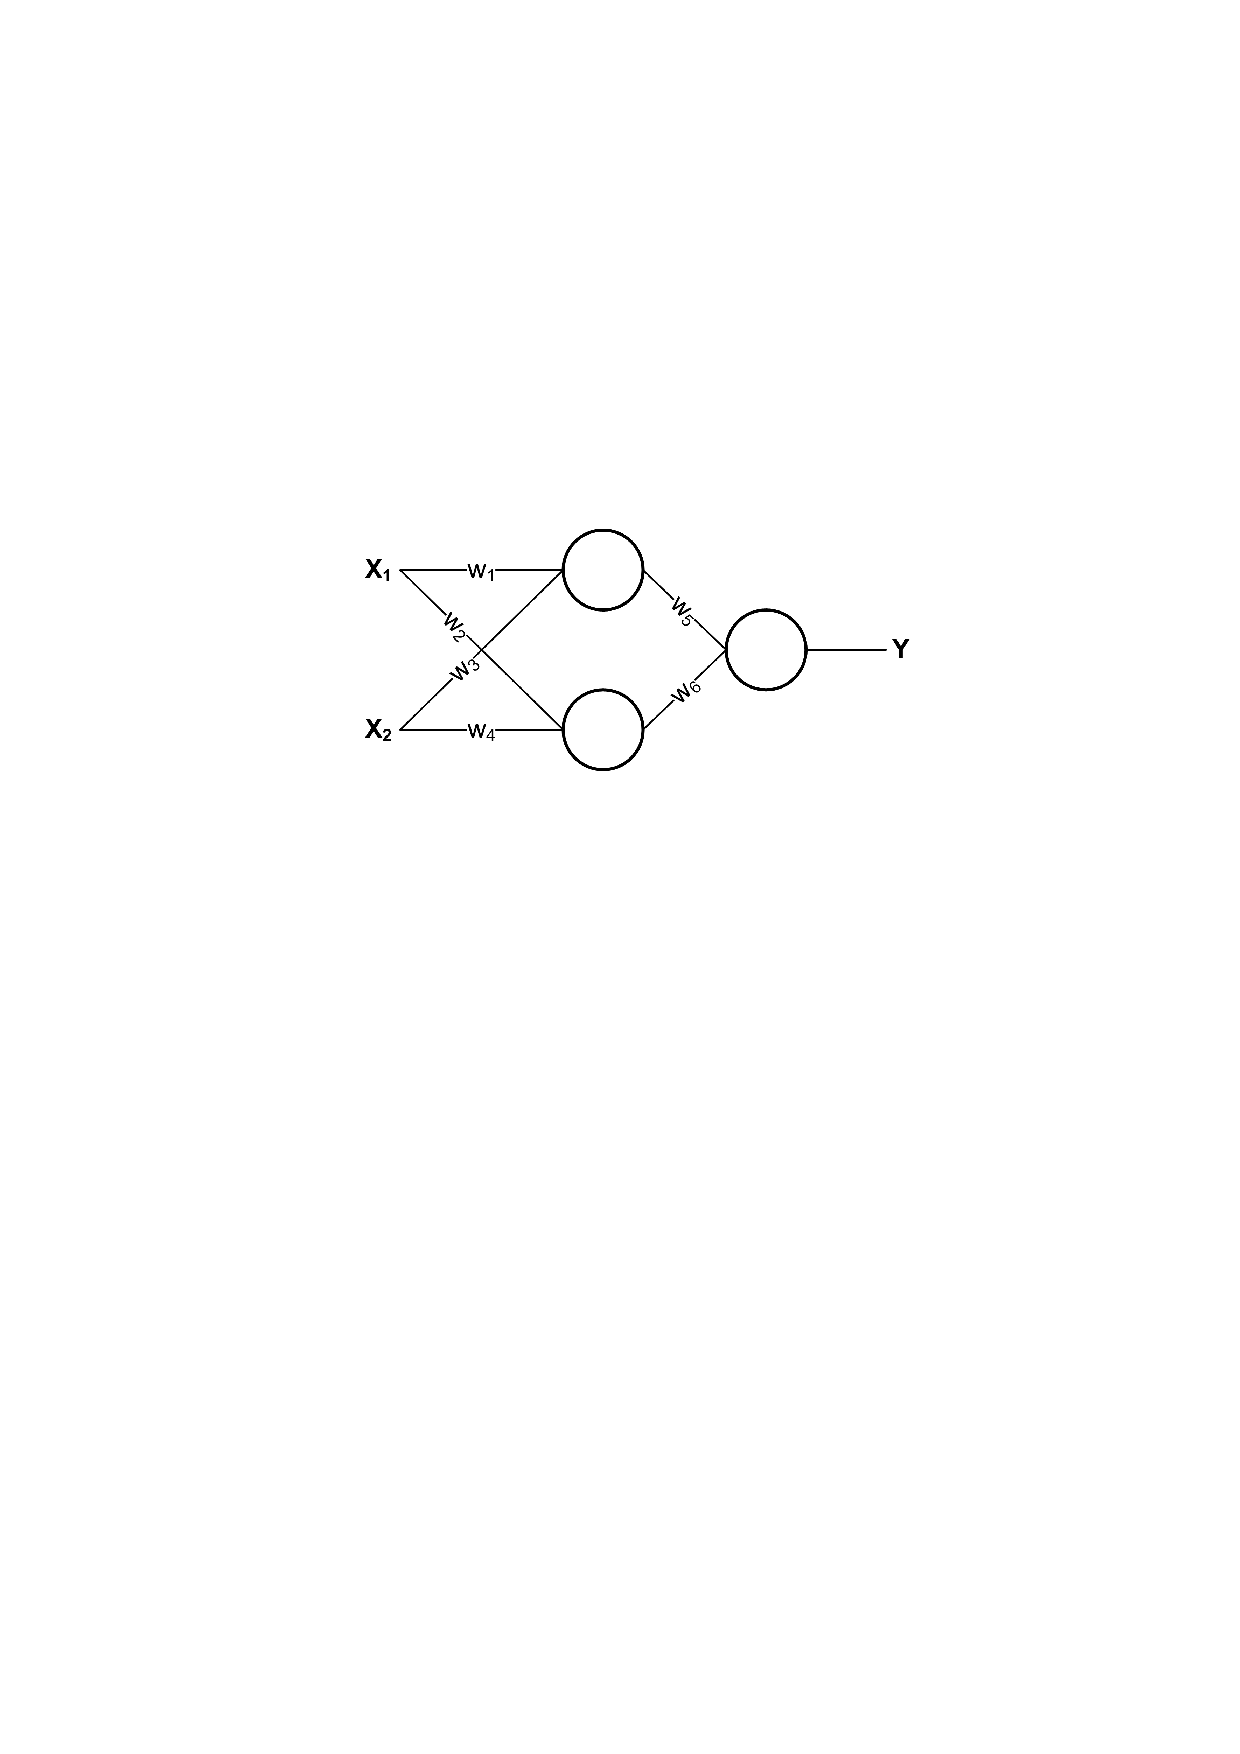
\includegraphics[width=0.5\textwidth]{Figure/nn}\\
  \caption{A two-layer neural network.}\label{nn}
\end{figure}

\subsection{Convolutional neural networks}

\begin{enumerate}
\item Count the total number of parameters in LeNet (pp.46, slides of Lecture.8). How many parameters in all of the convolutional layers? How many parameters in all of the fully-connected layers?
    
    {\color{red} 
    Note:
    \begin{enumerate}
    \item The filter size of each convolutional and pooling(subsampling) layer: \\
    %
    C1: $5\times 5$ (i.e., each unit of C1 has a $5\times 5$ receptive field in its preceding layer);\\
    S2: $2\times 2$;\\
    C3: $5\times 5$;\\
    S4: $2\times 2$;
    \item Fully-connected layers in LeNet include C5, F6, and OUTPUT
    \end{enumerate}
    }

\item In a convolutional layer the units are organized into planes, each of which is called a feature map. The units within a feature map (indexed $q$) have different inputs, but all share a common weight vector, $\bm{w}^{(q)}$. A convolutional network is usually trained through backprorogation. Let $J^{(q)}$ be the number of units in the $q$th feature map, $z_{j}^{(q)}$ the activation of the $j$th unit, $x_{ji}^{(q)}$ the $i$th input for the $j$th unit, $w_i^{(q)}$ the $i$th element of $\bm{w}^{(q)}$, $L$ the training loss. Derive the gradient of $w_{i}^{(q)}$.
\end{enumerate}

\subsection{Gradient vanishing/explosion}

In this problem we will study the difficulty of back-propagation in training deep neural networks. For simplicity, we consider the simplest deep neural network: one with just a single neuron in each layer, where the output of the neuron in the $j$th layer is $z_j = \sigma(a_j) = \sigma(w_jz_{j-1}+b_j)$. Here $\sigma$ is some activation function whose derivative on $x$ is $\sigma'(x)$. Let $m$ be the number of layers in the neural network, $L$ the training loss.

\begin{enumerate}
\item Derive the derivative of $L$ w.r.t. $b_1$ (the bias of the neuron in the first layer).
\item Assume the activation function is the usual sigmoid function $\sigma(x) = 1/(1+\exp\{-x\})$. The weights $\bm{w}$ are initialized to be $|w_j| < 1\ (j=1,\dots,m)$.
    \begin{enumerate}
    \item Explain why the above gradient ($\partial L/\partial b_1$) tends to vanish ($\to 0$) when $m$ is large.
    \item Even if $|w|$ is large, the above gradient would also tend to vanish, rather than explode ($\to\infty$). Explain why. (A rigorous proof is not required.)
    \end{enumerate}
\item One of the approaches to (partially) address the gradient vanishing/explosion problem is to use the rectified linear (ReL) activation function instead of the sigmoid. The ReL activation function is $\sigma(x) = \max\{0, x\}$. Explain why ReL can alleviate the gradient vanishing problem as faced by sigmoid.
\item A second approach to (partially) address the gradient vanishing/explosion problem is layer-wise pre-training. Restricted Boltzemann machine (RBM) is one of the widely-used models for layer-wise pre-training. Figure~\ref{rbm} shows an example of RBM which includes $K$ hidden units $\bm{h}$, and $J$ input units $\bm{v}$. Let us define the joint distribution as the following general form:
\begin{align}
P(\bm{v}, \bm{h}) = \frac{1}{Z}\exp\left( \sum_{i}\theta_{i}\phi_{i}(\bm{v},\bm{h}) \right),
\end{align}
where $Z=\sum_{\bm{v},\bm{h}}\exp\left( \sum_{i}\theta_{i}\phi_{i}(\bm{v},\bm{h}) \right)$ is the normalization term; $\phi_{i}(\bm{v},\bm{h})$ are some features; $\theta_{i}$ are the parameters corresponding to the weights in the RBM. Consider the simplest learning algorithm, gradient descent. Show that
\begin{align}
\frac{\partial \log P(\bm{v})}{\partial \theta_{i}} = \sum_{\bm{h}}\phi_{i}(\bm{v},\bm{h})P(\bm{h}|\bm{v}) - \sum_{\bm{v},\bm{h}}\phi_{i}(\bm{v},\bm{h})P(\bm{v},\bm{h}).
\end{align}
\end{enumerate}

\begin{figure}[!htp]
  \centering
  % Requires \usepackage{graphicx}
  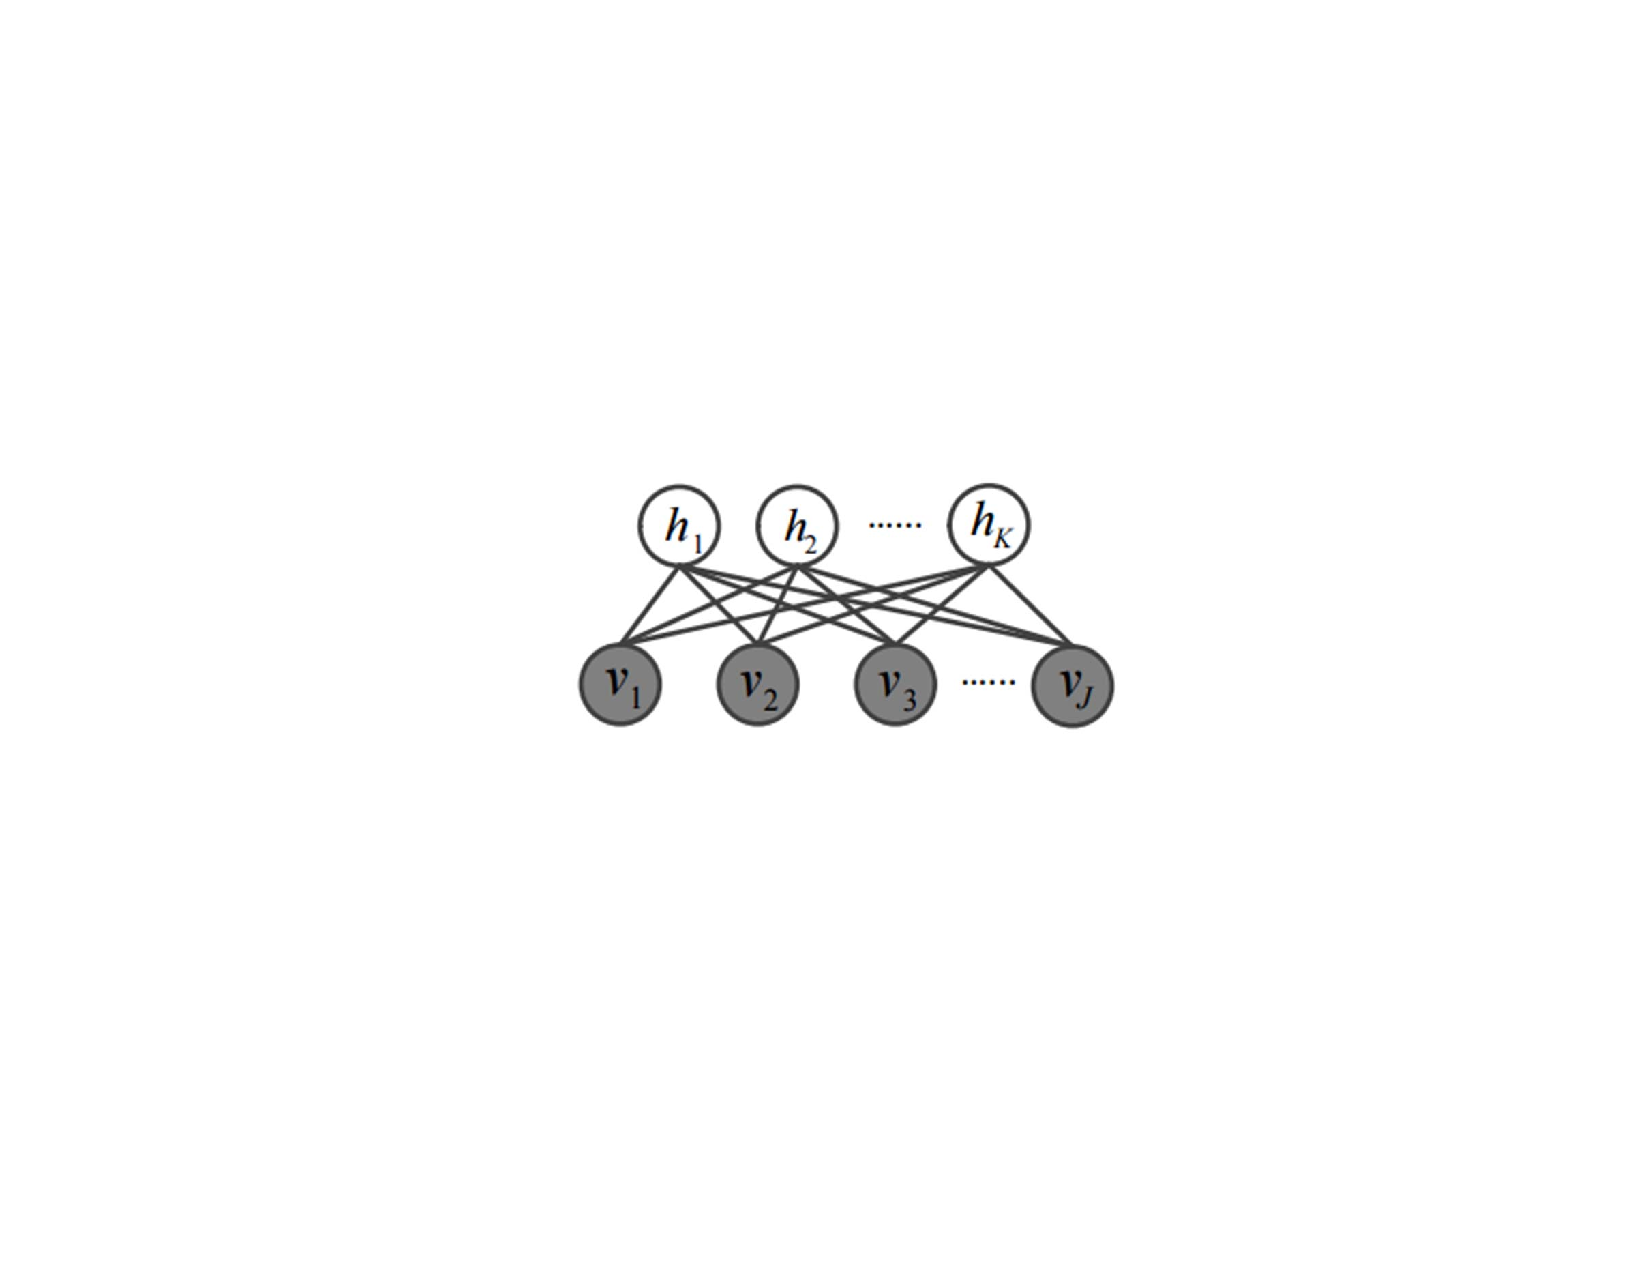
\includegraphics[width=0.4\textwidth]{Figure/rbm} \\
  \caption{A restricted Boltzmann machine.}\label{rbm}
\end{figure}

\section{Support Vector Machines (50 Points) (Yuntian)}
\subsection{Support Vector Regression (25 Points)}
We now extend support vector machines (SVM) to regression problems. Recall that in regression problems, we have $n$ data points $(x_i,y_i)_{i=1}^n$ where $x_i\in \mathbb{R}^m$ and $y_i\in \mathbb{R}$. Given a function class $\mathcal{F}$ (\eg linear or quadratic functions), we want to fit a function $f\in\mathcal{F}$ on the training set:
\begin{align}
f^\star = \argmin_{f\in\mathcal{F}}\, C\sum_{i=1}^n l(f(x_i),y_i) + R(f)
\end{align}
where $l(\cdot, \cdot)$ is the loss function, $R(f)$ is the regularization term, $C$ controls the regularization strength. The first part tries to fit data, and the second part penalizes complex $f$ to avoid over-fitting.

In the support vector regression (SVR) framework, we consider linear function class $\mathcal{F}=\{x\to w^T x\}$ (we do not consider interception term for simplicity). We use $ \ell_2 $-regularizer $R(f) = \frac{1}{2}\|w\|_2^2$ for $f(x)=w^T x$. For the loss function $l$, similar to the hinge-loss function in SVM classification, we employ an $\epsilon$-insensitive error function
\begin{align}
l_{\epsilon}(f(x),y) =
\begin{cases}
0       &      \quad {\textrm{if } |f(x)-y| < \epsilon}\\
|f(x)-y|-\epsilon     &      \quad {\textrm{otherwise}}.
\end{cases}
\end{align}
Then we get the following optimization problem:
\begin{align}
w^\star = \argmin_w\, C \sum_{i=1}^n l_\epsilon(w^T x_i,y_i) + \frac{1}{2}\|w\|_2^2.
\end{align}
\begin{enumerate}
\item Write down the dual problem of SVR. (Hint: follow the derivations for SVM)
\item Write down the KKT conditions, and explain what are the ``support vectors''.
\item Derive a kernelized version of SVR. For a test point $x$, write down the prediction rule.
\item Give one reason why do we usually solve the dual problem of SVR and SVM instead of the primal.
\item Implement SVR on a \href{http://www.cs.cmu.edu/~epxing/Class/10701-15F/files/SVR_dataset.txt}{1-D toy dataset}. Each line of the dataset contains a training instance $(x_i,y_i)$ (separated by a tab). For this problem, you need to
    \begin{itemize}
    \item Use RBF kernel $k(x_i,x_j) = \exp(-\frac{\|x_i-x_j\|_2^2}{2h^2})$, and take $h=0.5${\color{red}, $C=4$, $\epsilon=0.1$}.
    \item Plot the prediction curve for $x\in[0,1]$ and show the support vectors versus other training points in the training dataset.
    \end{itemize}
    (Hint: You are allowed to use optimization toolkits such as CVX or Matlab's inbuilt function quadprog to solve the dual problem.)
\end{enumerate}
\subsection{Support Kernel Machines (20 Points)}
In SVM, the kernel function can be viewed as a similarity measure between data points. In some classification scenarios, features may come from different sources or modalities, e.g. in some tasks the data may contain both image features and text features. In that case, since these are different representations, they have different measures of similarity corresponding to different kernels. In such a case, we want to learn a combination of kernels instead of using a single kernel. There is significant amount of work in combing kernels, here we adapt the notations in \cite{bach2004multiple}.

We begin by considering a linear case of Support Kernel Machine (SKM). Suppose the data points $x_i\in\mathcal{X}=\mathbb{R}^k$. We also assume we are given a decomposition of $\mathbb{R}^k=\mathbb{R}^{k_1}\times\cdots\times\mathbb{R}^{k_m}$, so that each data point $x_i$ can be decomposed into $m$ block components, i.e. $x_i=(x_{1i},\cdots,x_{mi})$ where each $x_{ji}$ is in general a vector. In real tasks, each block may correspond to a certain kind of representation, e.g. $x_{1i}$ may correspond to image features and $x_{2i}$ may be text features.

Our goal is to find a linear classifier of the form $y=\textrm{sign}(w^Tx+b)$ where $w$ has the same block decomposition $w=(w_1,\cdots,w_m)\in\mathbb{R}^{k_1+\cdots+k_m}$. Recall that in linear SVM the objective is:
\begin{align}
\mini_{\substack{w \in \mathbb{R}^{k_1}\times\cdots\times\mathbb{R}^{k_m} \\
\xi_i\ge0, \ 
b\in\mathbb{R}}} & \quad \frac{1}{2}\|w\|_2^2+C\sum_{i=1}^n\xi_i \\
\subto & \quad y_i(\sum_j w_j^T x_{ji}+b)\ge 1-\xi_i, \ \forall i \in\{1,\cdots,n\}
\end{align}
In SKM, we encourage the sparsity of the vector $w$ at the level of blocks. The primal problem for the SKM is defined as:
\begin{align}
\mini_{\substack{w \in \mathbb{R}^{k_1}\times\cdots\times\mathbb{R}^{k_m} \\ \xi_i\ge0, \ b\in\mathbb{R}}} 
& \quad \frac{1}{2}(\sum_{j=1}^m d_j \|w_j\|_2)^2+C\sum_{i=1}^n\xi_i\\
\subto & \quad y_i(\sum_j w_j^T x_{ji}+b)\ge 1-\xi_i, \ \forall i \in\{1,\cdots,n\}
\end{align}
where $d_j>0$ can be seen as constant.
\begin{enumerate}
\item By introducing dual variables $\alpha_i\ge 0$ and $\beta_i\ge 0$, we get the Lagrangian function
\begin{align}
\mathcal{L} = \frac{1}{2} (\sum_{j=1}^m d_j\|w_j\|_2)^2 + C\sum_{i=1}^n\xi_i - \sum_{i=1}^n \alpha_i (y_i(\sum_{j=1}^m w_j^Tx_{ji}+b)-1+\xi_i) - \sum_{i=1}^n\beta_i\xi_i
\end{align}
Denote $\gamma = \sum_{j=1}^m d_j \|w_j\|_2$.
\begin{enumerate}[(a)]
\item Show that at the {\color{red}minimum} of the Lagrangian function, {\color{red}i.e. $w = \argmin_w \mathcal{L}$ for this and the following questions},
\begin{align}
\|w_j\|_2 d_j \gamma = w_j^T \sum_{i=1}^n \alpha_i y_i x_{ji}, \ \forall j\in\{1,\cdots,m\}
\end{align}
\item Show that $\|\sum_{i=1}^n \alpha_i y_i x_{ji}\|_2\le d_j \gamma$, $\forall j\in\{1,\cdots,m\}$.

{\color{red}Note: for (b) you can get full credit if you only consider $w_j\neq 0$, but you can get 5 extra points if you include $w_j=0$ case in your proof. A hint is that $\mathcal{L}$ is not differentiable w.r.t. $w_j$ if $w_j=0$, and you may refer to \href{http://www.eecs.berkeley.edu/~wainwrig/ee227a/ee227a_subgradient_lecture.pdf}{this link} for how to deal with that case by using $\partial \|x\|_2 = \{g:\|g\|_2\le 1\}$ if $x=0$.}
\item Show that
\begin{itemize}
\item if $\|\sum_i \alpha_i y_i x_{ji}\|_2< d_j \gamma$, then $w_j=0$,
\item if $\|\sum_i \alpha_i y_i x_{ji}\|_2= d_j \gamma$, then $\exists \eta_j>0$, such that $w_j = \eta_j \sum_i \alpha_i y_i x_{ji}$.
\end{itemize}
\end{enumerate}
\item Recall from homework 2 that $ \ell_1 $ norm can encourage sparsity. Explain the effect of the regularization term $\frac{1}{2}(\sum_{j=1}^m d_j \|w_j\|_2)^2$.
\item Now we extend the above analysis to a kernelized version. Assume that we have a mapping $\phi:\mathcal{X}\to\mathbb{R}^f$ which is generally a non-linear function. We assume that $\phi(x)$ has $m$ block components $\phi(x)=(\phi_1(x),\cdots,\phi_m(x))${\color{red}, and we also assume $w$ has the same decomposition $w=(w_1,\cdots,w_m)$}. Show that at the {\color{red}minimum} of the Lagrangian function, $\exists\eta_j\ge0$ such that $w_j=\eta_j \sum_{i=1}^n\alpha_iy_i\phi_j(x_i)$.
\end{enumerate}
\subsection{SVM Error Analysis (5 Points)}
In this problem, we want to analyze the error of SVM classification. Assume that we have $n$ data points $(x_i,y_i)_{i=1}^n$ where $x_i\in \mathbb{R}^m$ and $y_i={1,\cdots,K}$. Assume that we train an SVM classifier $f_{(x_1,y_1),\cdots(x_n,y_n)}$ on these $n$ data points.

For a randomly drawn test data point $(x_{n+1},y_{n+1})$, the prediction is $y_{n+1}^{\rm pred} = f_{(x_1,y_1),\cdots,(x_n,y_n)}(x_{n+1})$. We assume that the $n$ training data points and the test data point $(x_{n+1},y_{n+1})$ are drawn i.i.d from some unknown underlying distribution. The expected error rate is defined as:
\begin{align}
{\sf err} = \mathbb{E}_{(x_1,y_1),\cdots(x_n,y_n)} \mathbb{E}_{(x_{n+1},y_{n+1})} [\one\cbb{f_{(x_1,y_1),\cdots,(x_n,y_n)}(x_{n+1})\neq y_{n+1}}]
\end{align}
where the indicator function $\one\cbb{A} = 1 $ if $ A $ is true, otherwise 0. 
\begin{enumerate}
\item Show the the expected error rate is equal to the expectation of leave-one-out cross validation error for $n+1$ data points.
\item In the lecture, we have the statement that ``the leave-one-out cross-validation error does not depend on the dimensionality of the feature space but only on the number of support vectors''. Show that this statement is true by explaining why
\begin{align}
{\sf err}_{\rm loocv} \le \frac{n_s}{n+1}
\end{align}
where ${\sf err}_{\rm loocv}$ is the leave-one-out cross-validation error for training set $(x_i,y_i)_{i=1}^{n+1}$, $n_s$ is the number of support vectors.
\end{enumerate}

\bibliographystyle{plain}
\bibliography{main}

\end{document}
